\documentclass{beamer}
\usepackage[latin1]{inputenc}
\usepackage{graphicx}
\usetheme{Warsaw}

\title{Sage Math Extension - Chrome Extension}
\author{T. Turner}\institute{University of Washington}

\begin{document}

\begin{frame}
\titlepage

\end{frame}

\begin{frame}
This is the first module of the Sage Math Extension
\\~\\
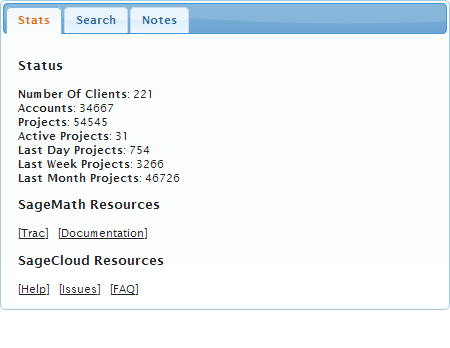
\includegraphics[width=.9\textwidth]{mod1.png}
\end{frame}
\begin{frame}
The Stats module shows the live status of the Sage Math Cloud server (Salvus). For more on Salvus: \href{http://salvusmath.blogspot.com/2012/12/what-is-salvus-i-started-salvus-project.html}{\beamergotobutton{Link}}
\\~\\
This module uses Javascript, JSON, and WebSockets to communicate with a Sage Math distributed node.js server. A JSON request is sent for the current stats, a reply is parsed and printed to the document. These starts are refreshed everytime you open the Sage Math Extension.
\\~\\
Lastly, some Sage Math resource links are available for quick access.
\end{frame}

\begin{frame}
This is the second module of the Sage Math Extension
\\~\\
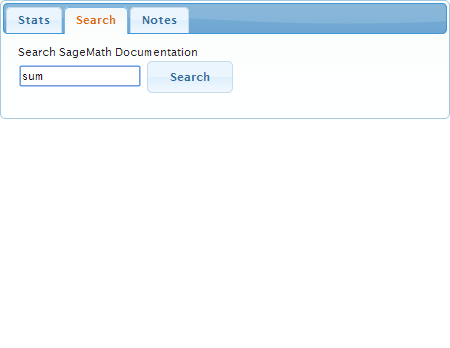
\includegraphics[width=.9\textwidth]{mod2.png}
\end{frame}

\begin{frame}
The second module provides quick access to the online Sage Math documentation.
\\~\\
Any terms entered here are passed directly to the same action page as Sage Math's search form when the "Search" button is clicked.
\\~\\
Additional search locations could be added, or a parsed set of results with scrollability!
\end{frame}

\begin{frame}
This is the third module of the Sage Math Extension
\\~\\
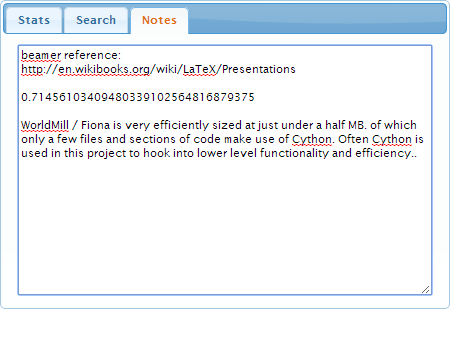
\includegraphics[width=.9\textwidth]{mod3.png}
\end{frame}

\begin{frame}
The third module provides an easy access place to save notes and other information.
\\~\\
Information can be entered in the same way as any web text field. The module uses your browser's local storage to store the information. The information is saved automatically on each key stroke (and in some other cases as well, but this mechanism is not fully complete).
\\~\\
Additional functionality is in the works, examples:
\begin{itemize}
\item Save notes as .txt
\item Remote storage
\item Share (image, pastebin, email, etc)
\end{itemize}
\end{frame}

\end{document}
%sagemathcloud={"zoom_width":90}